We now recall below the expression for the experimental cross section, \eqref{eq:DVPiPCrossSection_exp}

        \begin{equation*}
          \recallLabel{eq:DVPiPCrossSection_exp}.
        \end{equation*}

The experimental data as described in \chref{Chapter:Experiment} provides access to $N(Q^2,x_B,t,\phi_{\pi})$ and \Lumiint, while the data simulated as described in \chref{Chapter:Simulations} allows determination of the correction factors. The specific steps for calculating these terms that are explained in this chapter are: 


\begin{itemize}
  \item Correct for experimental and simulation deficiencies in pre-processing \secref{sec:Ch4_data_preprocess}
  \item Select \dvpip events from experimental and simulated data \secref{sec:Ch4_event_selection}
  \item Determine integrated luminosity from accumulated beam charge \secref{sec:luminosity}
  \item Partition data into kinematic bins \secref{sec:Ch4_binning}
  \item Apply correction factors and calculate uncertainties \secref{sec:Ch4_corr_factors}
\end{itemize}

Cross section results are presented in \secref{sec:Ch4_cross_section}. This analysis method\footnote{Analysis repository is found here:  \href{https://github.com/robertej19/clas12DVPiP}{https://github.com/robertej19/clas12DVPiP}}
  yields a binned \xsec with correction factors applied bin-by-bin. This approach is favored for its straightforwardness, but comes at the cost of additional uncertainties. Statistical methods to supplant this are discussed in \secref{sec:Ch5_IBU}. 


\section{Data Pre-Processing}\label{sec:Ch4_data_preprocess}
    
In a perfect world, experimental and simulated data could be immediately utilized to compute cross-sections once obtained. In reality, a variety of factors - such as defects in experimental detectors or issues in modeling real-world physics - necessitate minor adjustments to be made to the datasets. It is of course not feasible to re-run entire experiments just to address these small issues, and instead is best handled by pre-processing the data with well-motivated correcting factors.  In particular, the experimental data requires fiducial cuts corresponding to detector dead-zones or otherwise problematic areas, as well as energy loss corrections due to underestimates in the reconstruction scheme. The simulated datasets require smearing factors to more closely resemble the real-world detector and reconstruction algorithm performances.


\subsection{Experimental Data Pre-Processing}\label{sec:momcorr}
     %\subsubsection{Momentum Corrections}{Mom Corr}
%\subsubsection{Energy Loss Corrections}
Charged particles lose energy via ionization and radiation along their paths. Reconstruction schemes attempt to correct for this, but issues can remain in various situations. The electron reconstruction showed negligible deviations from expected performance. The proton reconstruction exhibited a two-band structure due to detector topology, as shown in \ref{fig:protoncorra}. The issue was deeply studied by S. Lee, who developed and implemented a correction scheme \parencite{Lee2022MeasurementDetector}. We demonstrate in \ref{fig:protoncorrb} the correction is functioning as expected in this work. 


    \begin{figure}[H]
        \centering
        
        \subfloat[Distribution without correction. \label{fig:protoncorra}]{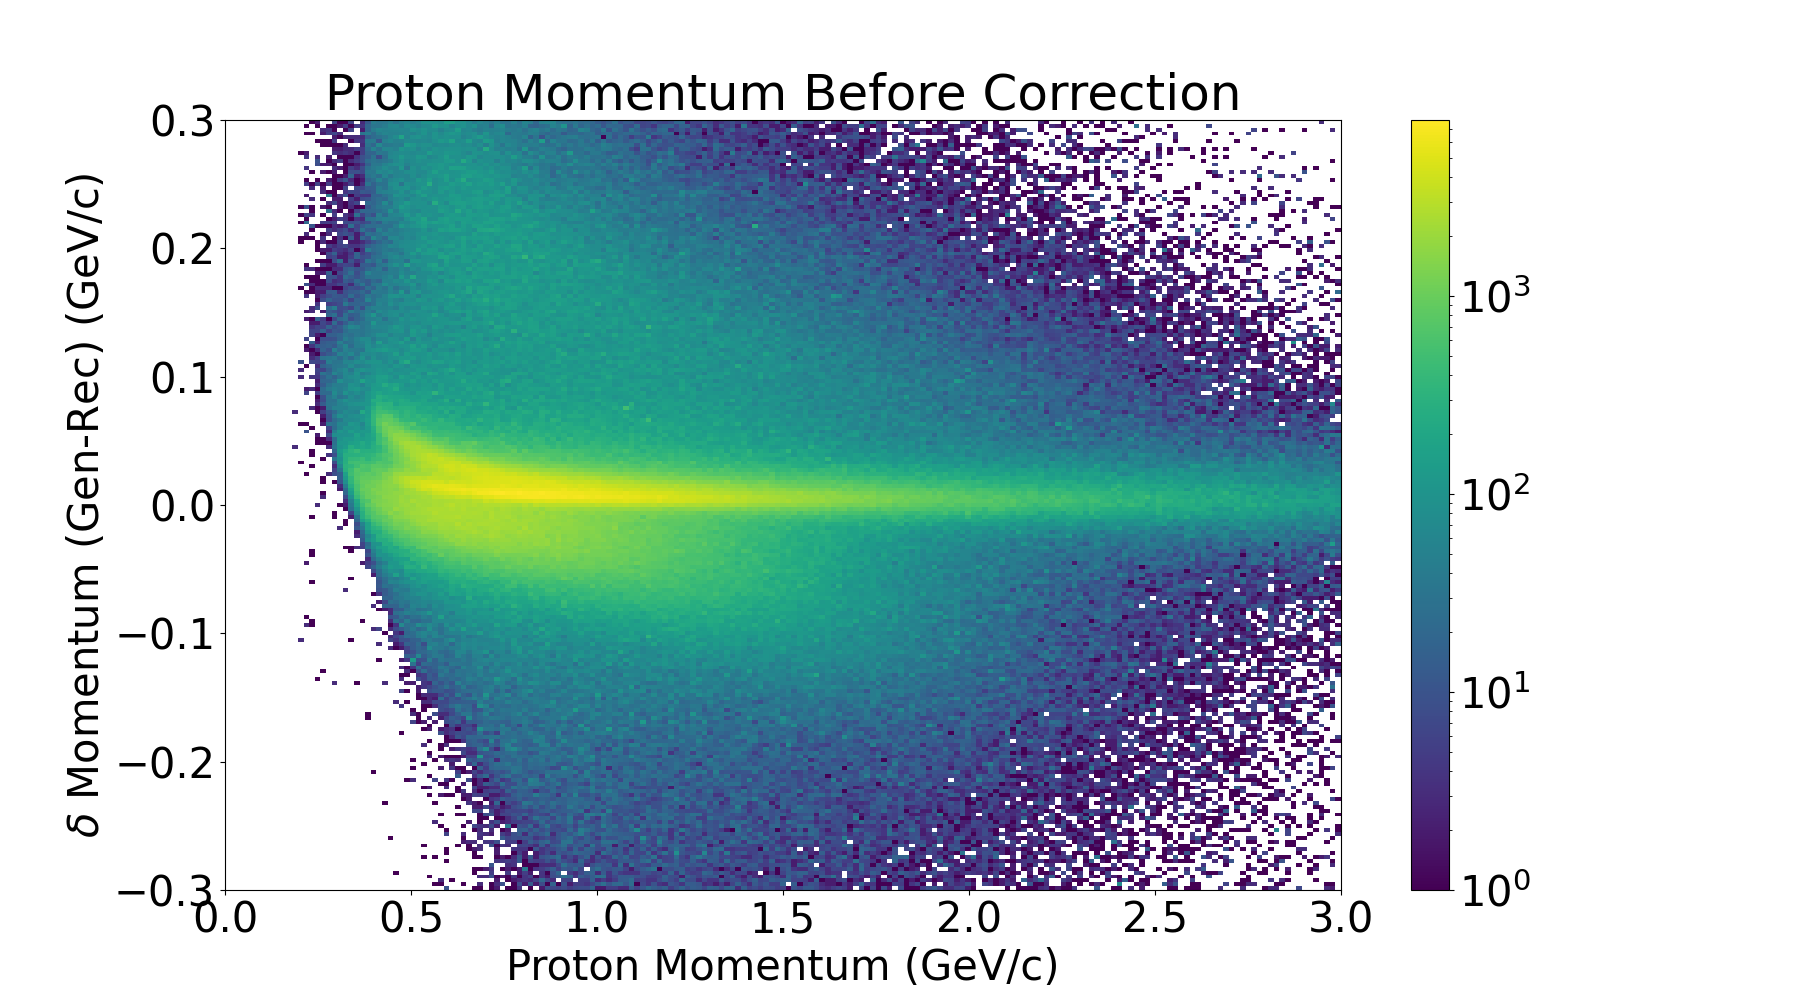
\includegraphics[trim={0 0 5cm 0},clip,width=0.5\textwidth]{Chapters/Ch4-BaseAnalysis/0_preprocessing/0_A_experimental_data_preprocessing/pics/noneProton_Momentum_Before_Correction.png}}
        \hfill
        \subfloat[Distribution with correction. \label{fig:protoncorrb}]{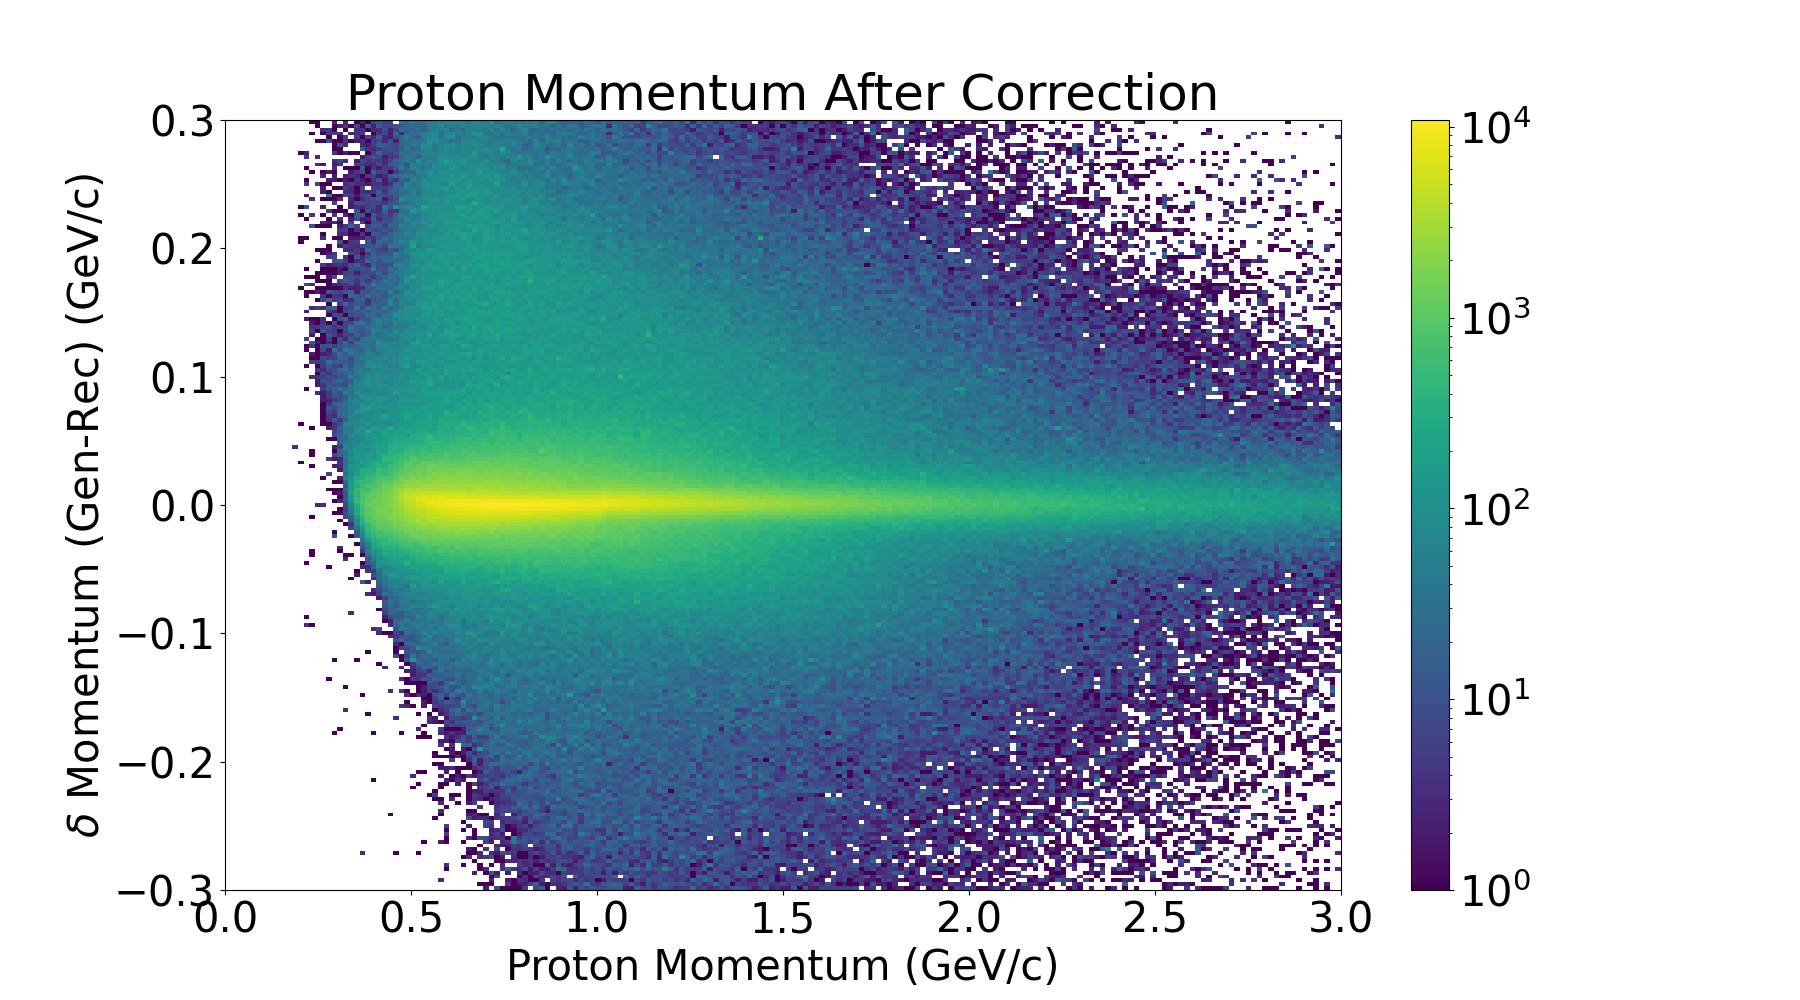
\includegraphics[trim={0 0 5cm 0},clip,width=0.5\textwidth]{Chapters/Ch4-BaseAnalysis/0_preprocessing/0_A_experimental_data_preprocessing/pics/noneProton_Momentum_After_Correction.png}}
    
        \caption[Proton Momentum Correction]{Difference between generated and reconstructed proton momentum as a function of proton momentum, before (a) and after (b) momentum corrections are implemented.}\label{fig:protoncorr}
    \end{figure}

\iffalse
A charged particle loses its energy through its passage through material via ionization
and radiation

We first corrected the energy loss of the proton using the simulation data. After
applying the proton loss corrections to the experimental data and the simulation, we
reduced the reconstruction bias by correcting the single particle kinematics in the
experimental data. To match the resolution, the kinematics of the simulated data
was smeared.

\fi
     
\subsection{Simulation Data Pre-Processing}\label{sec:momsmear}
   %\subsubsection{Simulation:Experiment Resolution Matching}

The detector responses in the GEMC system were modeled to perform slightly better than their real-world counterparts. This means the signal data from the simulations is cleaner than the real experiment, and so smearing factors must be added to provide a better match. This convention was chosen because the alternative (with simulations performing worse than real-world detectors) would yield data that is difficult to deconvolve. \figref{fig:bad} shows the discrepancy between the experimental and simulated data sets, for various variable combinations. 

\begin{figure}[hbt]
	\centering
	\includegraphics[page=125,width=0.3\linewidth]{Chapters/Ch4-BaseAnalysis/0_preprocessing/0_B_simulation_data_preprocessing/pics/nosmear/outbending_rad_All_All_All_no_smearingME_epgg_exp_vs_sim.png}
	\includegraphics[page=123,width=0.3\linewidth]{Chapters/Ch4-BaseAnalysis/0_preprocessing/0_B_simulation_data_preprocessing/pics/nosmear/outbending_rad_All_All_All_no_smearingMM2_egg_exp_vs_sim.png}
	\includegraphics[page=128,width=0.3\linewidth]{Chapters/Ch4-BaseAnalysis/0_preprocessing/0_B_simulation_data_preprocessing/pics/nosmear/outbending_rad_All_All_All_no_smearingMM2_epgg_exp_vs_sim.png}
	\includegraphics[page=130,width=0.3\linewidth]{Chapters/Ch4-BaseAnalysis/0_preprocessing/0_B_simulation_data_preprocessing/pics/nosmear/outbending_rad_All_All_All_no_smearingMM2_ep_exp_vs_sim.png}
	\includegraphics[page=133,width=0.3\linewidth]{Chapters/Ch4-BaseAnalysis/0_preprocessing/0_B_simulation_data_preprocessing/pics/nosmear/outbending_rad_All_All_All_no_smearingMpi0_exp_vs_sim.png}
	\includegraphics[page=135,width=0.3\linewidth]{Chapters/Ch4-BaseAnalysis/0_preprocessing/0_B_simulation_data_preprocessing/pics/nosmear/outbending_rad_All_All_All_no_smearingMPt_exp_vs_sim.png}
	
	\caption[Simulation and Experiment Matching before Smearing]{Comparison of experiment (blue) and simulation (red) missing mass, energy, momentum, and invariant gamma-gamma mass distributions, before any smearing factors were added to the simulation data.}
	\label{fig:bad}
\end{figure}


To improve the matching between simulation and experiment, Gaussian smearing factors were added after reconstruction to the simulated dataset. These factors were tuned by S. Lee \parencite{Lee2022MeasurementDetector} to have optimal matching across all missing mass spectra combinations \figref{fig:good}. In particular, the outgoing proton and photon momenta were smeared with Gaussian kernels with standard deviations $\sigma$ determined as function of momenta and dependent on particle location (CD, FD, or FT).

\begin{figure}[hbt]
	\centering
	\includegraphics[page=125,width=0.3\linewidth]{Chapters/Ch4-BaseAnalysis/0_preprocessing/0_B_simulation_data_preprocessing/pics/yessmear/outbending_rad_All_All_All_for_aps_2022_plots_sangcutsME_epgg_exp_vs_sim.png}
	\includegraphics[page=123,width=0.3\linewidth]{Chapters/Ch4-BaseAnalysis/0_preprocessing/0_B_simulation_data_preprocessing/pics/yessmear/outbending_rad_All_All_All_for_aps_2022_plots_sangcutsMM2_egg_exp_vs_sim.png}
	\includegraphics[page=128,width=0.3\linewidth]{Chapters/Ch4-BaseAnalysis/0_preprocessing/0_B_simulation_data_preprocessing/pics/yessmear/outbending_rad_All_All_All_for_aps_2022_plots_sangcutsMM2_epgg_exp_vs_sim.png}
	\includegraphics[page=130,width=0.3\linewidth]{Chapters/Ch4-BaseAnalysis/0_preprocessing/0_B_simulation_data_preprocessing/pics/yessmear/outbending_rad_All_All_All_for_aps_2022_plots_sangcutsMM2_ep_exp_vs_sim.png}
	\includegraphics[page=133,width=0.3\linewidth]{Chapters/Ch4-BaseAnalysis/0_preprocessing/0_B_simulation_data_preprocessing/pics/yessmear/outbending_rad_All_All_All_for_aps_2022_plots_sangcutsMpi0_exp_vs_sim.png}
	\includegraphics[page=135,width=0.3\linewidth]{Chapters/Ch4-BaseAnalysis/0_preprocessing/0_B_simulation_data_preprocessing/pics/yessmear/outbending_rad_All_All_All_for_aps_2022_plots_sangcutsMPt_exp_vs_sim.png}
	
	\caption[Simulation and Experiment Matching after Smearing]{Comparison of experiment (blue) and simulation (red) missing mass, energy, momentum, and invariant gamma-gamma mass distributions, with smearing factors added to the simulation data proton and photon momenta.}
	\label{fig:good}
\end{figure}





    \clearpage
    
\section{Event Selection}\label{sec:Ch4_event_selection}
    Overview words about event selection

\subsection{Exclusivity Cuts}\label{sec:eventselection}

    \begin{wrapfigure}{r}{0.58\textwidth}
    	\vspace*{-0.3cm}
    	\includegraphics[page=10,width=0.97\linewidth]{Chapters/Ch4-BaseAnalysis/1_Event_Selection_Cuts/figures/eppi0.exclusive.pdf}
    	\caption{MM$^2$ (epX) vs $\theta_X\pi$ 2D distribution.}
    	\label{fig:MM2vsThetaXPi}
    \end{wrapfigure}
    After the selection of events with at least one electron, proton and two photons, it is time to take a look at the exclusive distributions.
    The Fig.~\ref{fig:MM2vsThetaXPi} shows 2D distribution of MM$^2$ (epX) vs $\theta_{X\pi}$, where MM$^2$ (epX) is a missing mass squared of (epX) system and should have a peak near 0.0182 GeV$^2$, and $\theta_{X\pi}$ is an angle between expected and reconstructed pion.
    The bright spot on the figure corresponds to the exclusive $ep\rightarrow~ep\pi^0$ events.
    In order to reduce the background exclusivity cuts  need to be developed based on the conservation of energy and momentum.
    The relevant 1D exclusive distributions are shown on the Fig.~\ref{fig:rawexclusive1} and \ref{fig:rawexclusive2}.
    
    \begin{figure}[hbt]
    	\centering
    	\includegraphics[page=4,width=0.47\linewidth]{Chapters/Ch4-BaseAnalysis/1_Event_Selection_Cuts/figures/eppi0.exclusive.pdf}
    	\includegraphics[page=5,width=0.47\linewidth]{Chapters/Ch4-BaseAnalysis/1_Event_Selection_Cuts/figures/eppi0.exclusive.pdf}
    	\caption{Exclusive distributions for events with at least one electron, proton and two photons.}
    	\label{fig:rawexclusive1}
    \end{figure}
    
    \begin{figure}[hbt]
    	\centering
    	\includegraphics[page=6,width=0.47\linewidth]{Chapters/Ch4-BaseAnalysis/1_Event_Selection_Cuts/figures/eppi0.exclusive.pdf}
    	\includegraphics[page=8,width=0.47\linewidth]{Chapters/Ch4-BaseAnalysis/1_Event_Selection_Cuts/figures/eppi0.exclusive.pdf}
    	\caption{Exclusive distributions for events with at least one electron, proton and two photons.}
    	\label{fig:rawexclusive2}
    \end{figure}
    
    \subsubsection{Tight \texorpdfstring{$M_{\gamma\gamma} $} mass and transverse missing momenta cuts}
    
    The first step is to use tighter $\gamma\gamma$ mass cut: $0.096<M_{\gamma\gamma}<0.168$ GeV, and take a look at the missing transverse momentum distributions (see Fig.~\ref{fig:ptdistributions}).
    From momentum conservation law we expect transverse momentum to be zero, so we can apply cuts on $\Delta p_x$ and $\Delta p_y$ to further improve exclusive channel selection.
    The cuts $|\Delta p_x|<0.2$ and $|\Delta p_y|<0.2$ correspond roughly to 4-5 $\sigma$.
    
    \begin{figure}[hbt]
    	\centering
    	\includegraphics[page=24,width=0.47\linewidth]{Chapters/Ch4-BaseAnalysis/1_Event_Selection_Cuts/figures/eppi0.exclusive.pdf}
    	\includegraphics[page=25,width=0.47\linewidth]{Chapters/Ch4-BaseAnalysis/1_Event_Selection_Cuts/figures/eppi0.exclusive.pdf}
    	\caption{Exclusive distributions for events with at least one electron, proton and two photons.}
    	\label{fig:ptdistributions}
    \end{figure}
    
    The exclusive distributions after tight $M_{\gamma\gamma}$ mass and transverse missing momenta cuts are shown on Fig.~\ref{fig:rawexclusive3} and display much stronger signal peaks on top of reduced background.
    
    \begin{figure}[hbt]
    	\centering
    	\includegraphics[page=43,width=0.45\linewidth]{Chapters/Ch4-BaseAnalysis/1_Event_Selection_Cuts/figures/eppi0.exclusive.pdf}
    	\includegraphics[page=44,width=0.45\linewidth]{Chapters/Ch4-BaseAnalysis/1_Event_Selection_Cuts/figures/eppi0.exclusive.pdf}
    	\includegraphics[page=45,width=0.45\linewidth]{Chapters/Ch4-BaseAnalysis/1_Event_Selection_Cuts/figures/eppi0.exclusive.pdf}
        \includegraphics[page=47,width=0.45\linewidth]{Chapters/Ch4-BaseAnalysis/1_Event_Selection_Cuts/figures/eppi0.exclusive.pdf}
    
    	\caption{Exclusive distributions after tight $M_{\gamma\gamma}$ mass and transverse missing momenta cuts .}
    	\label{fig:rawexclusive3}
    \end{figure}
    
    \subsubsection{\texorpdfstring{$\theta_{X\pi}$} cut determination}
    
    The cut on angle between expected and reconstructed pion is used in order to further reduce background.
    To choose the value of the $\theta_{X\pi}$ cut the $MM^2(epX)$ distribution is analyzed at multiple $\theta_{X\pi}$ cut values and fit using gaussian+polynomial function as shown on Fig.~\ref{fig:mm2fordifferenttheta}.
    From the fit we can estimate the number of good exclusive events (gaussian) and the number of background events (polynomial) and their dependence on $\theta_{X\pi}$ cut.
    Fig.~\ref{fig:sigbgvsthetacutQ2} and~\ref{fig:sigbgvsthetacutxB} show the numbers of signal and background events as functions of $\theta_{X\pi}$ cut value for multiple bins in $Q^2$ and $x_B$.
    These plots show that the cut $\theta_{X\pi}<2^\circ$ allows to select the most number of good events with the least background, and relaxing it beyond $2^\circ$ does not gain us any good exclusive events but increases background.
    
    
    \begin{figure}[hbt]
    	\centering
    	\includegraphics[page=123,width=0.3\linewidth]{Chapters/Ch4-BaseAnalysis/1_Event_Selection_Cuts/figures/sigbg_eppi0.pdf}
    	\includegraphics[page=125,width=0.3\linewidth]{Chapters/Ch4-BaseAnalysis/1_Event_Selection_Cuts/figures/sigbg_eppi0.pdf}
    	\includegraphics[page=128,width=0.3\linewidth]{Chapters/Ch4-BaseAnalysis/1_Event_Selection_Cuts/figures/sigbg_eppi0.pdf}
    	\includegraphics[page=130,width=0.3\linewidth]{Chapters/Ch4-BaseAnalysis/1_Event_Selection_Cuts/figures/sigbg_eppi0.pdf}
    	\includegraphics[page=133,width=0.3\linewidth]{Chapters/Ch4-BaseAnalysis/1_Event_Selection_Cuts/figures/sigbg_eppi0.pdf}
    	\includegraphics[page=135,width=0.3\linewidth]{Chapters/Ch4-BaseAnalysis/1_Event_Selection_Cuts/figures/sigbg_eppi0.pdf}
    	
    	\caption{$MM^2(epX)$ distributions for multiple $\theta_{X\pi}$ cut values.}
    	\label{fig:mm2fordifferenttheta}
    \end{figure}
    
    
    \begin{figure}[hbt]
    	\centering
    	
    	\includegraphics[width=0.32\linewidth,page=34]{Chapters/Ch4-BaseAnalysis/1_Event_Selection_Cuts/figures/sigbg_eppi0.pdf}
    	\includegraphics[width=0.32\linewidth,page=51]{Chapters/Ch4-BaseAnalysis/1_Event_Selection_Cuts/figures/sigbg_eppi0.pdf}
    	\includegraphics[width=0.32\linewidth,page=68]{Chapters/Ch4-BaseAnalysis/1_Event_Selection_Cuts/figures/sigbg_eppi0.pdf}
    	\includegraphics[width=0.32\linewidth,page=85]{Chapters/Ch4-BaseAnalysis/1_Event_Selection_Cuts/figures/sigbg_eppi0.pdf}
    	\includegraphics[width=0.32\linewidth,page=102]{Chapters/Ch4-BaseAnalysis/1_Event_Selection_Cuts/figures/sigbg_eppi0.pdf}
    	\includegraphics[width=0.32\linewidth,page=119]{Chapters/Ch4-BaseAnalysis/1_Event_Selection_Cuts/figures/sigbg_eppi0.pdf}
    	
    	\caption{The numbers of signal (red markers) and background (black markers) events as functions of $\theta_{X\pi}$ cut value for multiple $Q^2$ bins.}
    	\label{fig:sigbgvsthetacutQ2}
    \end{figure}
    
    
    \begin{figure}[hbt]
    	\centering
    	
    	\includegraphics[width=0.32\linewidth,page=136]{Chapters/Ch4-BaseAnalysis/1_Event_Selection_Cuts/figures/sigbg_eppi0.pdf}
    	\includegraphics[width=0.32\linewidth,page=153]{Chapters/Ch4-BaseAnalysis/1_Event_Selection_Cuts/figures/sigbg_eppi0.pdf}
    	\includegraphics[width=0.32\linewidth,page=170]{Chapters/Ch4-BaseAnalysis/1_Event_Selection_Cuts/figures/sigbg_eppi0.pdf}
    	\includegraphics[width=0.32\linewidth,page=187]{Chapters/Ch4-BaseAnalysis/1_Event_Selection_Cuts/figures/sigbg_eppi0.pdf}
    	\includegraphics[width=0.32\linewidth,page=204]{Chapters/Ch4-BaseAnalysis/1_Event_Selection_Cuts/figures/sigbg_eppi0.pdf}
    	
    	\caption{The numbers of signal (red markers) and background (black markers) events as functions of $\theta_{X\pi}$ cut value for multiple $x_B$ bins.}
    	\label{fig:sigbgvsthetacutxB}
    \end{figure}
    
    \clearpage
    
    \subsubsection{Final exclusivity cuts}
    
    The list of final exclusive cuts is following:
    \begin{itemize}
    	\item $\Delta p_x<0.2$ GeV
    	\item $\Delta p_y<0.2$ GeV
    	\item $\theta_{X\pi}<2^\circ$
    	\item $0.096<M_{\gamma\gamma}<0.168$ GeV
    	\item $MM^2(epX)<0.5$ GeV$^2$
    \end{itemize}
    
    Exclusive distributions after all exclusivity cut except $MM^2(epX)<0.5$ GeV are shown on Fig.~\ref{fig:finalexclusive}
    
    \begin{figure}[hbt]
    	\centering
    	
    	\includegraphics[page=82,width=0.32\linewidth]{Chapters/Ch4-BaseAnalysis/1_Event_Selection_Cuts/figures/eppi0.exclusive.pdf}
    	\includegraphics[page=83,width=0.32\linewidth]{Chapters/Ch4-BaseAnalysis/1_Event_Selection_Cuts/figures/eppi0.exclusive.pdf}
    	\includegraphics[page=84,width=0.32\linewidth]{Chapters/Ch4-BaseAnalysis/1_Event_Selection_Cuts/figures/eppi0.exclusive.pdf}
    	\caption{Exclusive distributions after all exclusivity cuts .}
    	\label{fig:finalexclusive}
    \end{figure}
    
    
    
    
    
    
    
    To arrive at a DVEP candidate event, we do the following
    
    
    Code flow:
    
    Consider a directory with n hipo files. For each hipo file, do the following.
    
    Read each file event by event, and do the following
    
    Check that the event has the proper databanks, and if not, go to teh next event.
    
    Get a list of all the electrons*, protons*, and photons* in the event
    
    *= links to most up to date PID methods
    
    for every electron in the event (always only one, at least in the skims, but not held to be one) do the following
    For every proton in the event, do the following
    
    Calculate some basic quantities and fill histograms
    
    for every permutation of pairs of photons in the event, do the following
    
    calculate various kinematic quantities, and pass to see if creates a viable pion* and a viable DVEP event*
    
    if so, fill relevant histograms and count as a DVEP event, otherwise skip to next event
    
    viable pion: 
    pion mass betwen 100 and 180 MeV
    pion momentum greater than 1.5 GeV
    angle (theta) between each photon and the electron to be greater than 8 degrees
    
    viable DVEP event:
    Q2 greater than 1
    W greater than 2
    difference between theta of missing 4-momentum and reconstructed pion less than 2 degrees
    difference between missing X px and py 300 MeV each or less
    Difference in missing mass squared between pion and X less than 1 GeV ** make sure this is right
    difference in missing energy and X less than 1 GeV **make sure this is right
    

\iffalse
\subsection{Kinematic Fitting}

    Instead of rigid cuts, we can use maximum likelihood estimators - include notes from Janet's class

    The first issue arises with event classification - although we want to examine events with a neutral pion (which decays
to two photons), a proton, and an electron, in practice we create a huge amount of data that is consistent with either pure
noise, or from other hadronic processes. We must classify each of the many millions of recorded events as either signal or
noise. This is traditionally done over the union of single parameter classifications with rigid boundaries as a box in parameter
space (e.g. a signal event is one which satisfies a strict set of conditions). Unfortunately, this excludes many valid events that
were reconstructed poorly in only one or a few of the many (roughly 20) different parameters under consideration. This firstly
reduces the data sample size, which is relatively expensive to obtain, and secondly introduces large systematic uncertainties
into the analysis. A more advanced approached is to use machine learning classifiers to improve event selection and decrease
signal uncertainty. This more advanced method of classification is currently being implemented and verified in the analysis to
demonstrate that it supplants the traditional method effectively


    \begin{table}[h]
        \centering
        \begin{tabular}{c|ccc}
            \textbf{Configuration} & \textbf{Gen. Type} & \textbf{Background} & \textbf{Nevents (MM)} \\ \hline
                & norad & none & 5 \\
                & norad & 50 nA & 5 \\
            Inbending & rad & 50 nA & 15 \\
                & rad & 45 nA & 10 \\
                & rad & 55 nA & 10 \\ \hline
                & norad & none & 10 \\
                & norad &  50 nA & 10 \\
            Outbending & rad & 50 nA & 30 \\
                 & rad & 40 nA & 10 \\
             & rad & 40 nA (+1.01) & 10 \\
            \hline
            Total & - & - & 1400 \\
        \end{tabular}
    \caption[Distribution of Simulated Events by Configuration]{Number of simulated events for various experimental configurations and conditions.\tabref{table:Generated_Data} shows the corresponding number of generated events per distribution. \textcolor{red}{\textbf{NOTE: Values in this table are placeholders and need to be updated with final figures}}}
    \label{table:simulated_data}
    \end{table}
\fi
    \clearpage
    
\section{Luminosity}\label{sec:luminosity}
    
%The strategy to calculate the luminosity is as follows:\\

% - For each run, retrieve a measure of how much beam passed through the target, I believe in the case of CLAS12 using the Faraday cup to measure beam charge
%    - sum the beam charge over all runs being considered and include any relevant corrections factors
%    - multiply this by target length, density, etc. to get the integrated luminosity
%    - use this value to calculate cross sections.

%Compare integrated luminosity of CLAS6 to CLAS12 (in 2011 analysis note)

Luminosity can calculated according to equation \ref{lumieq}
 \begin{equation}\label{lumieq}
            \Lumi = \frac{N_A l \rho Q_{FCUP}}{e}.
\end{equation}

$N_A$ is Avogadro's constant, l is the length of the target,  $\rho$ is the density of the target (liquid hydrogen), $Q_{FCUP}$ is the charge collected on the Faraday cup, and e is the charge of the electron. The values of these quantities are are as tabulated in table \ref{lumitable}. 


\begin{table}[h]
    \centering
    \begin{tabular}{rcc}
         %& Heading 1 & Heading 2 \\\hline
        Quantity & Symbol & CLAS12 Value \\\hline
       Avogadro's Number &  N$_A$  & 6.02214 x $10^{23}$ \\
        Electron Charge &e  &  1.602 x 10$^{-19}$ Coulombs \\
        Target Length &l &  5.00 cm \\
        Target Density &$\rho$  &  0.07 $g/cm^3$ (LH2) \\
        Charge on Faraday Cup & $Q_{FCUP}$ &  In data\\
    \end{tabular}
\caption[Terms of Luminosity Equation]{Values of terms in luminosity determination.}
\end{table}\label{lumitable}

The accumulated charge on the Faraday cup is calculated by taking the difference between the maximum and minimum values of beamQ for each run (events are not necessarily time ordered), and then summing these values. Typical runs at CLAS12 have an accumulated beam charge of tens to hundreds of thousands of nanoCoulombs. 

The Fall 2018 Inbending configuration integrated luminosity was calculated to be \Lumiint = 5.511802 x 10$^{40}$ $cm^{-2}$  = 5.511802 x 10$^{7}$  inverse femtobarns, and the Fall 2018 Outbending configuration was found to have \Lumiint = 4.651647 x 10$^{7}$ $fb^{-1}$



\iffalse
Implementation:
The bank \texttt{REC::Event} has an object \texttt{beamCharge}, in nanoCoulombs, which is described in the \texttt{DST} as ``beam charge integrated from the beginning of the run to the most recent reading of the gated Faraday Cup scaler in \texttt{RAW::scaler}, with slope/offset conversion to charge from CCDB. Note, this value will be zero in each file until the first scaler reading in that file.''. This is the (un?)gated beam charge. 


This can be accessed via:

\begin{lstlisting}
	def banknames = ['REC::Event','REC::Particle','REC::Cherenkov','REC::Calorimeter','REC::Traj','REC::Track','REC::Scintillator']

	if(banknames.every{event.hasBank(it)}) {
		def (evb,partb,cc,ec,traj,trck,scib) = banknames.collect{event.getBank(it)}
def fcupBeamCharge = evb.getFloat('beamCharge',0)
\end{lstlisting}

    According to \href{https://clas12.discourse.group/t/accessing-beam-charge-information/239}{this} we might need to use tag=1 RAW::scaler::fcupgated instead of REC::Event::beamCharge
\fi

    \clearpage
\section{Binning}\label{sec:Ch4_binning}
    To the author's knowledge, there is no singular mathematically optimized binning scheme criterion for a generalized 4-dimensional dataset. Concordantly, the multidimensional binning in this analysis was heuristically informed 


    \begin{figure}[H]
        \centering

        
        \subfloat[Inbending $xB$ vs. $Q^2$]{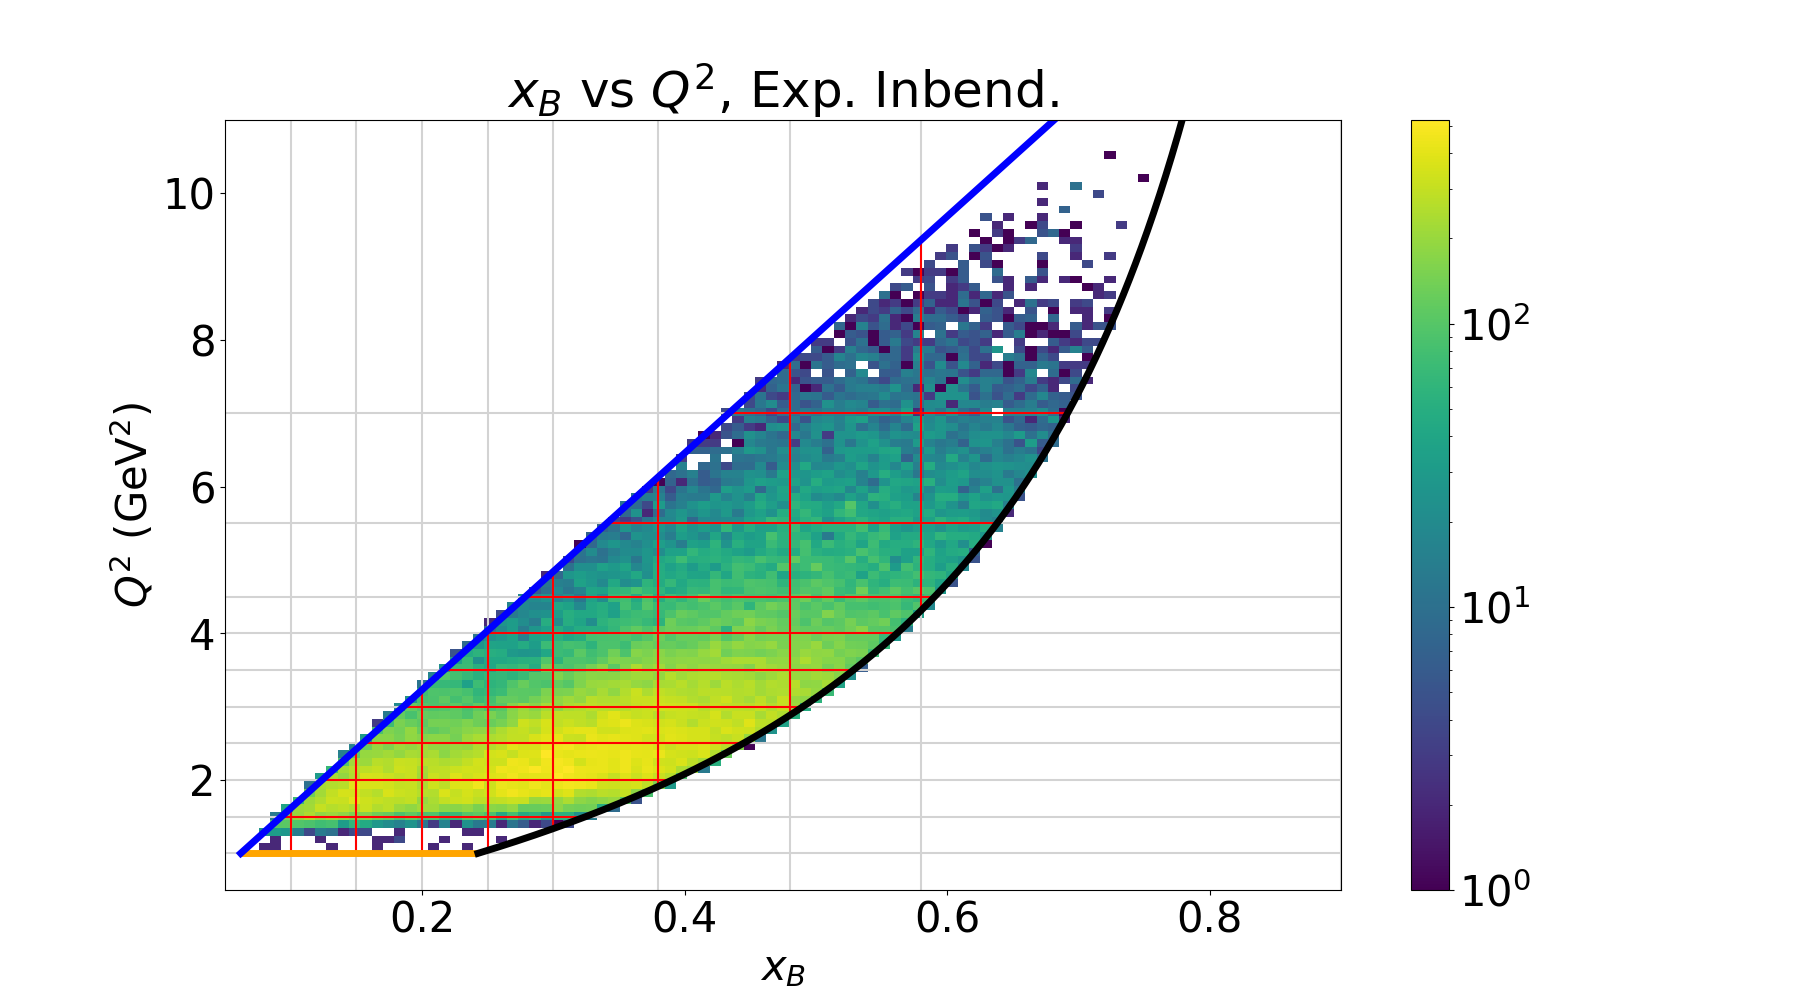
\includegraphics[trim={0 0 5cm 0},clip,width=0.5\textwidth]{Chapters/Ch4-BaseAnalysis/3_Binning/pics/x_B_vs_Q2,_Exp_Inbend.png}}
        \hfill
        \subfloat[Inbending $\phi$ vs. $t$]{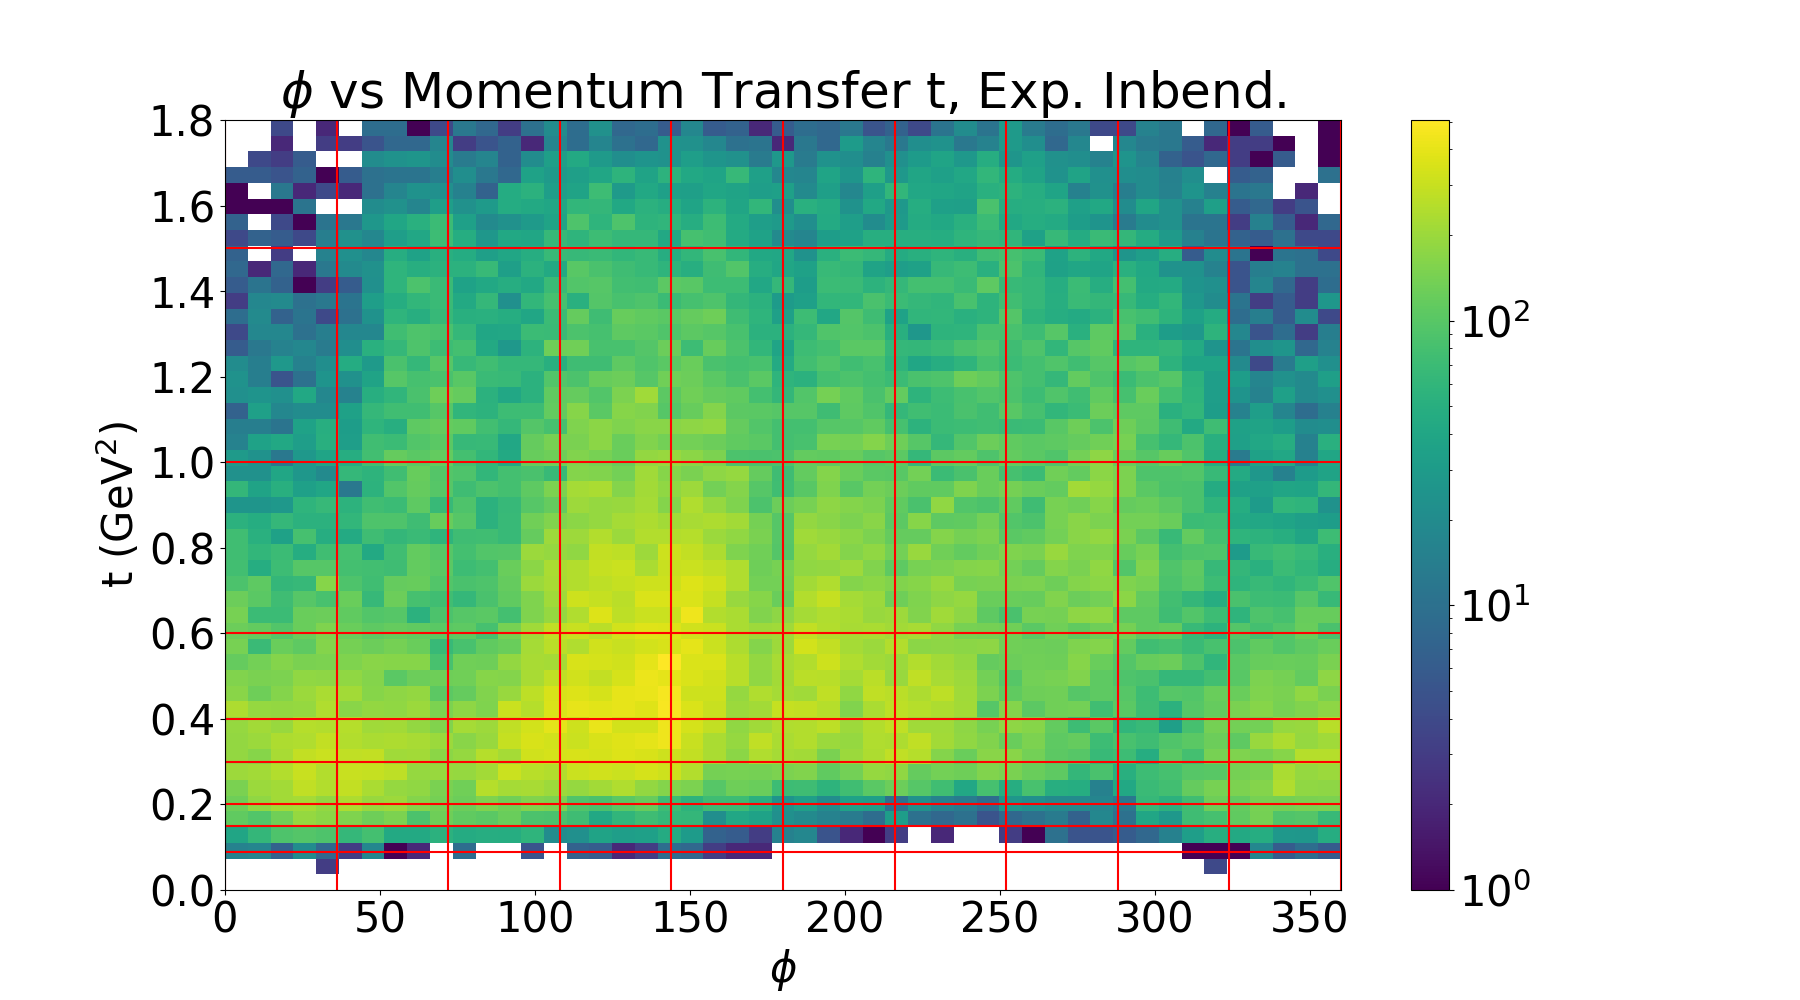
\includegraphics[trim={0 0 5cm 0},clip,width=0.5\textwidth]{Chapters/Ch4-BaseAnalysis/3_Binning/pics/phi_vs_Momentum_Transfer_t,_Exp_Inbend.png}}

        \subfloat[Outbending $xB$ vs. $Q^2$]{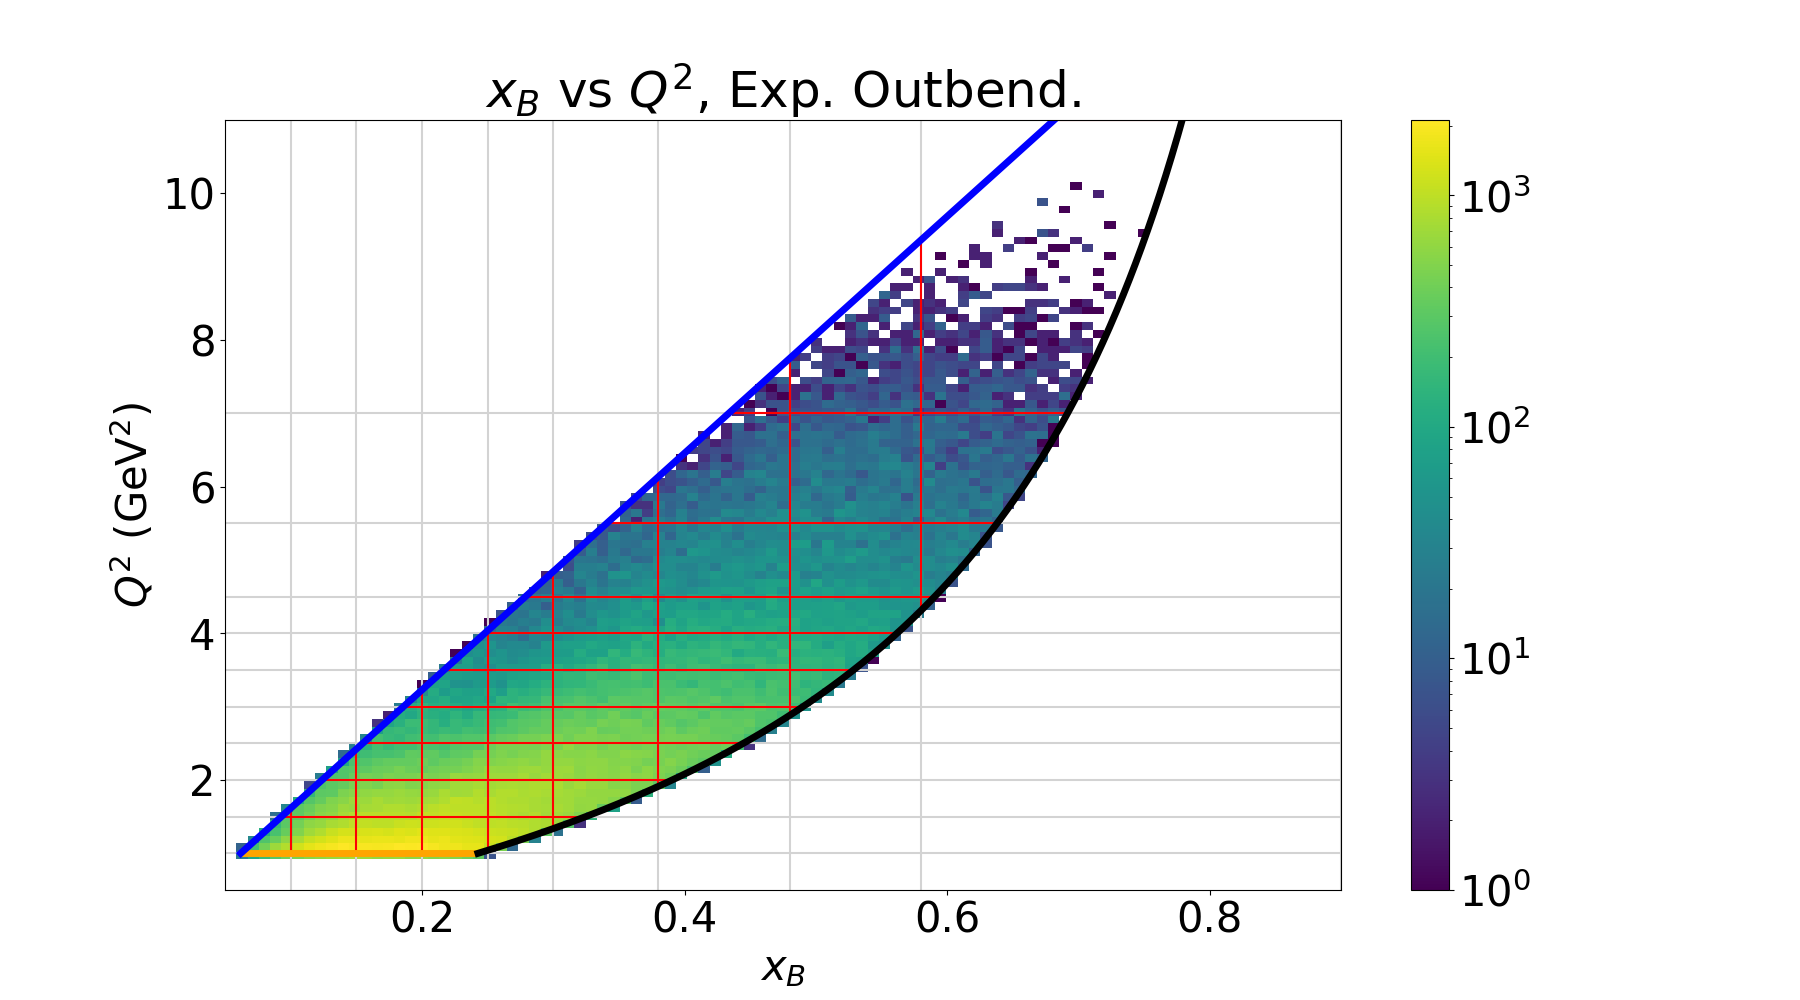
\includegraphics[trim={0 0 5cm 0},clip,width=0.5\textwidth]{Chapters/Ch4-BaseAnalysis/3_Binning/pics/x_B_vs_Q2,_Exp_Outbend.png}}
        \hfill
        \subfloat[Outbending $\phi$ vs. $t$]{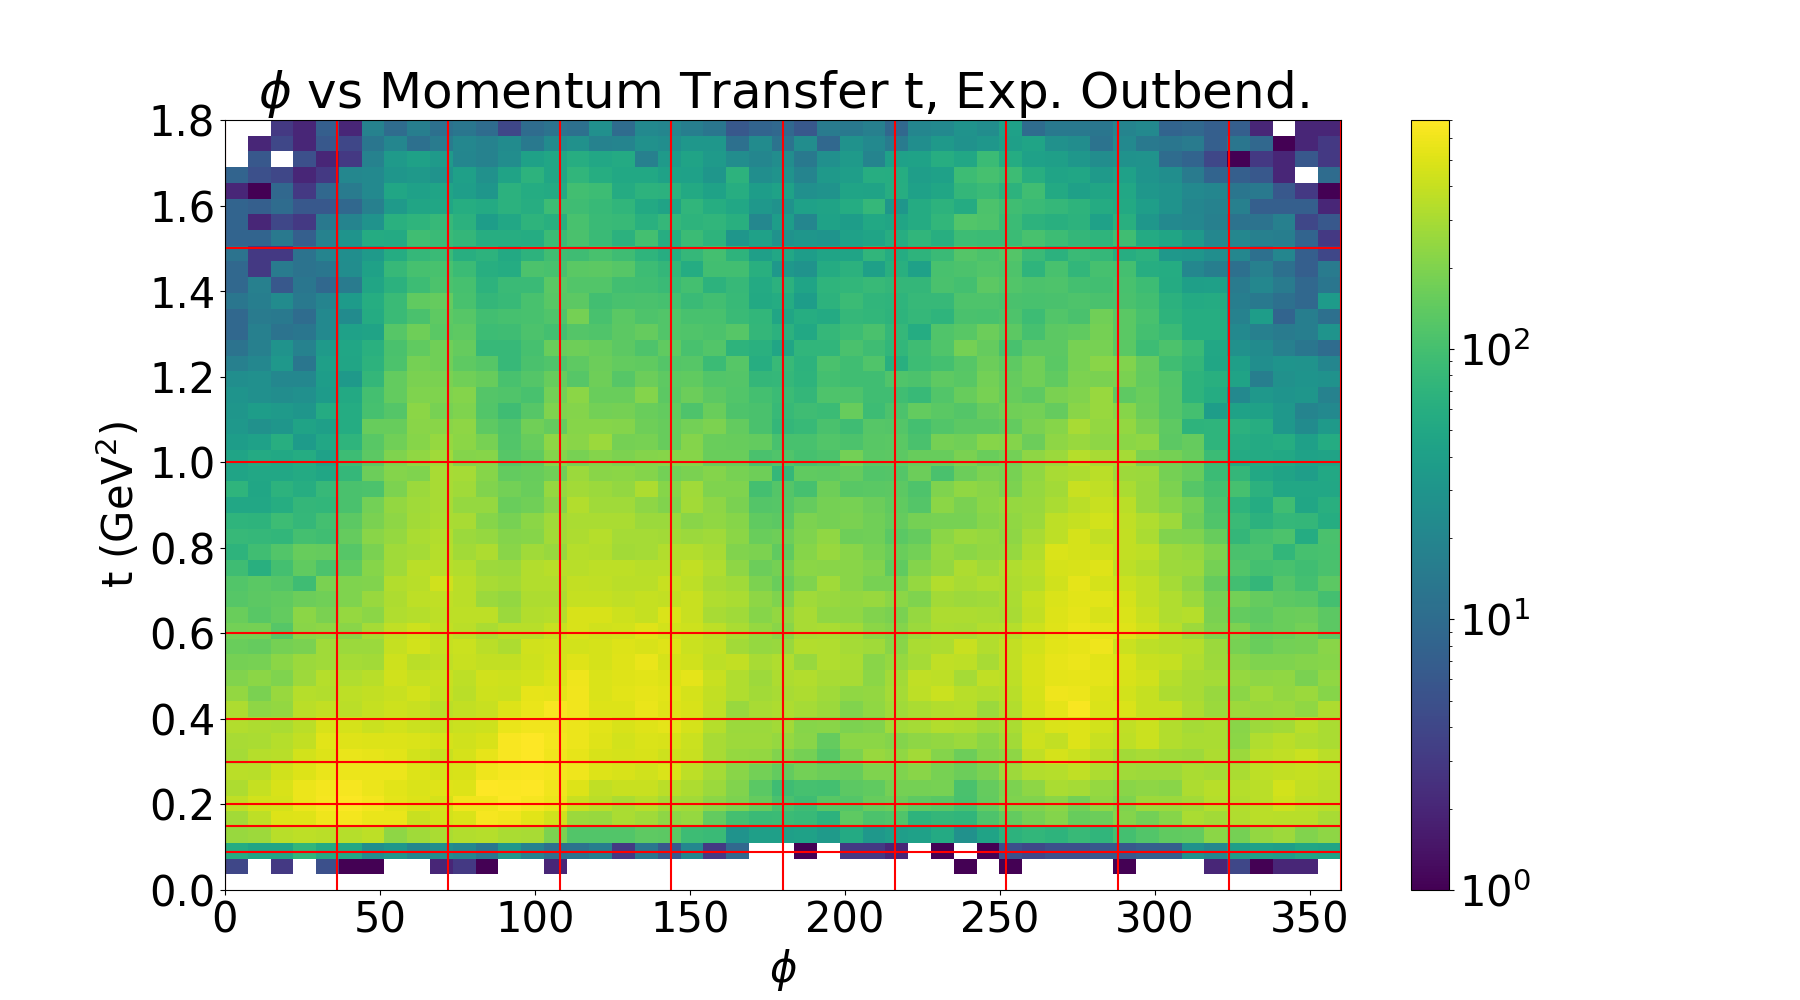
\includegraphics[trim={0 0 5cm 0},clip,width=0.5\textwidth]{Chapters/Ch4-BaseAnalysis/3_Binning/pics/phi_vs_Momentum_Transfer_t,_Exp_Outbend.png}}

        \caption[CLAS12 Data Binning Scheme]{Binning scheme for CLAS12 Fall 2018 Inbending (top row) and Fall 2018 Outbending (bottom row) datasets.}\label{fig:clas12_sub_portal}
    \end{figure}

Was chosen to overlap previous results \parencite{Bedlinskiy2014ExclusiveCLAS} to facilitate data comparisons. 

From equation 1.12

W2 = Q/x+m - Q = 4 -- Q = (4 - m) / (1/x - 1)

8.604^2 < q2
W >

 Q/x+m - Q >4

Q2< 74.028816





To avoid bin migration, set high q2 on generation.

\iffalse
Figure 5-19: The 2D histograms of events in ��2 and ���� for each configuration of final
level BH-DVCS events. The kinematic regions are bordered by the certain required
conditions: (1) ����′ > 2 GeV/c (green), (2) ��2 > 1 (GeV/c)2 (blue) and (3) �� > 2
GeV (red).

finite bin effects - center is not average  mean diff

bin volume correction - distribution cutoffs

It is important to choose an optimal multidimensional binning scheme for the cross
section extraction. In this thesis, the bin shape was designed to be a four dimensional
box. Some bins are not well fitted into the box due to the phase space condition. For
example, Fig. 5-19 shows several triangular bins in the ��2 −���� plane at the left side,
whose hypotenuse is determined by ����′ > 2 GeV/c.
The advantage of finer binning is to provide improved density estimation. The
acceptance corrections and the finite bin width effects should increase with the bin
size. However, the bin size cannot be narrower than the effective resolutions in the
binning variables to minimize bin migration. Extremely small bins would not have
any statistical significance in each bin, which would lead to an invalid analysis. It is
important to determine the optimal binning.


The different proton momentum thresholds were considered for the |��| binning.
The momentum thresholds required for the proton momentum reconstruction, 0.3
GeV/c for CD, 0.42 GeV/c for FD inbending, 0.5 GeV/c for FD outbending lead to
|��| threhsold of 0.09, 0.17 and 0.23 GeV2 respectively. To consider the bin migration
effect, the |��| bin was loosely set as [0.110, 0.150, 0.250, 0.400, 0.600, 0.800, 1.000]
GeV2. The number of events in the first bin was estimated with CD protons only.
Likewise, the FD outbending data was not used for the second bin event counting.
There are not enough statistics above |t|=1 GeV2 to determine the cross sections with
reasonable precision from the RG-A fall 2018 data alone.

The ��2−���� phase space was evenly divided by the bin edges [1.000, 1.200, 1.456,
1.912, 2.510, 3.295, 4.326, 5.761, 7.000] (GeV/c)2 and [0.062, 0.090, 0.118, 0.155,
0.204, 0.268, 0.357, 0.446, 0.581]. The ��2 − ���� bin boundaries are presented in
��2 − ���� plane with the 2D histogram of entire experimental data set in Fig. 5-19
with an explanation of the kinematics boundaries at the caption


The �� distributions are binned in equal width bins of width 15∘. Other possible
binning schemes include (1) the adjusted equal width binning to widen the bin width
at the central region to compensate for low statistics, and (2) the equal frequency

binning. The chosen binning scheme has three advantages; (1) the binning scheme is
symmetric with respect to �� = 180∘, (2) the frequency is directly translated into the
probability distribution in the same ��2 − ���� − |��| bin, and (3) it was used by other
experiments [107, 129].

\fi
    \clearpage
\section{Correction Factors and Uncertainty Analysis}\label{sec:Ch4_corr_factors}
    \subsection{Acceptance Correction}
The largest correction factor in this work is the acceptance correction, which is a convolution of detector efficiency, geometrical acceptance, reconstruction efficiency, and PID and event cuts. We defined acceptance in \eqref{eq:acceptance} as

    \begin{equation*}
      \recallLabel{eq:acceptance},
    \end{equation*}

where we utilize simulations to arrive at an estimator for the acceptance, $\hat{\epsilon}$. The correction term is calculated bin-by-bin, procedurally illustrated in \figref{fig:acccorr}. As defined, $\hat{\epsilon}$ is a product of geometrical acceptance, detector and reconstruction efficiencies, and fiducial and analysis (event selection) cuts, and values for this analysis were typically on the 1-10\% level. Low acceptance bins were excluded at a threshold of below 0.5\%. The distribution of acceptance correction factors is shown in \figref{fig:acccorrdist}. Statistical uncertainty was calculated based off counting statistics, and systematic uncertainty was estimated by changing the generator input model parameters by $\pm$ 10\% from their nominal values and comparing to the nominal run results. 

    \begin{figure}[H]
        \centering
        \subfloat[Raw counts $N_{exp}$.]{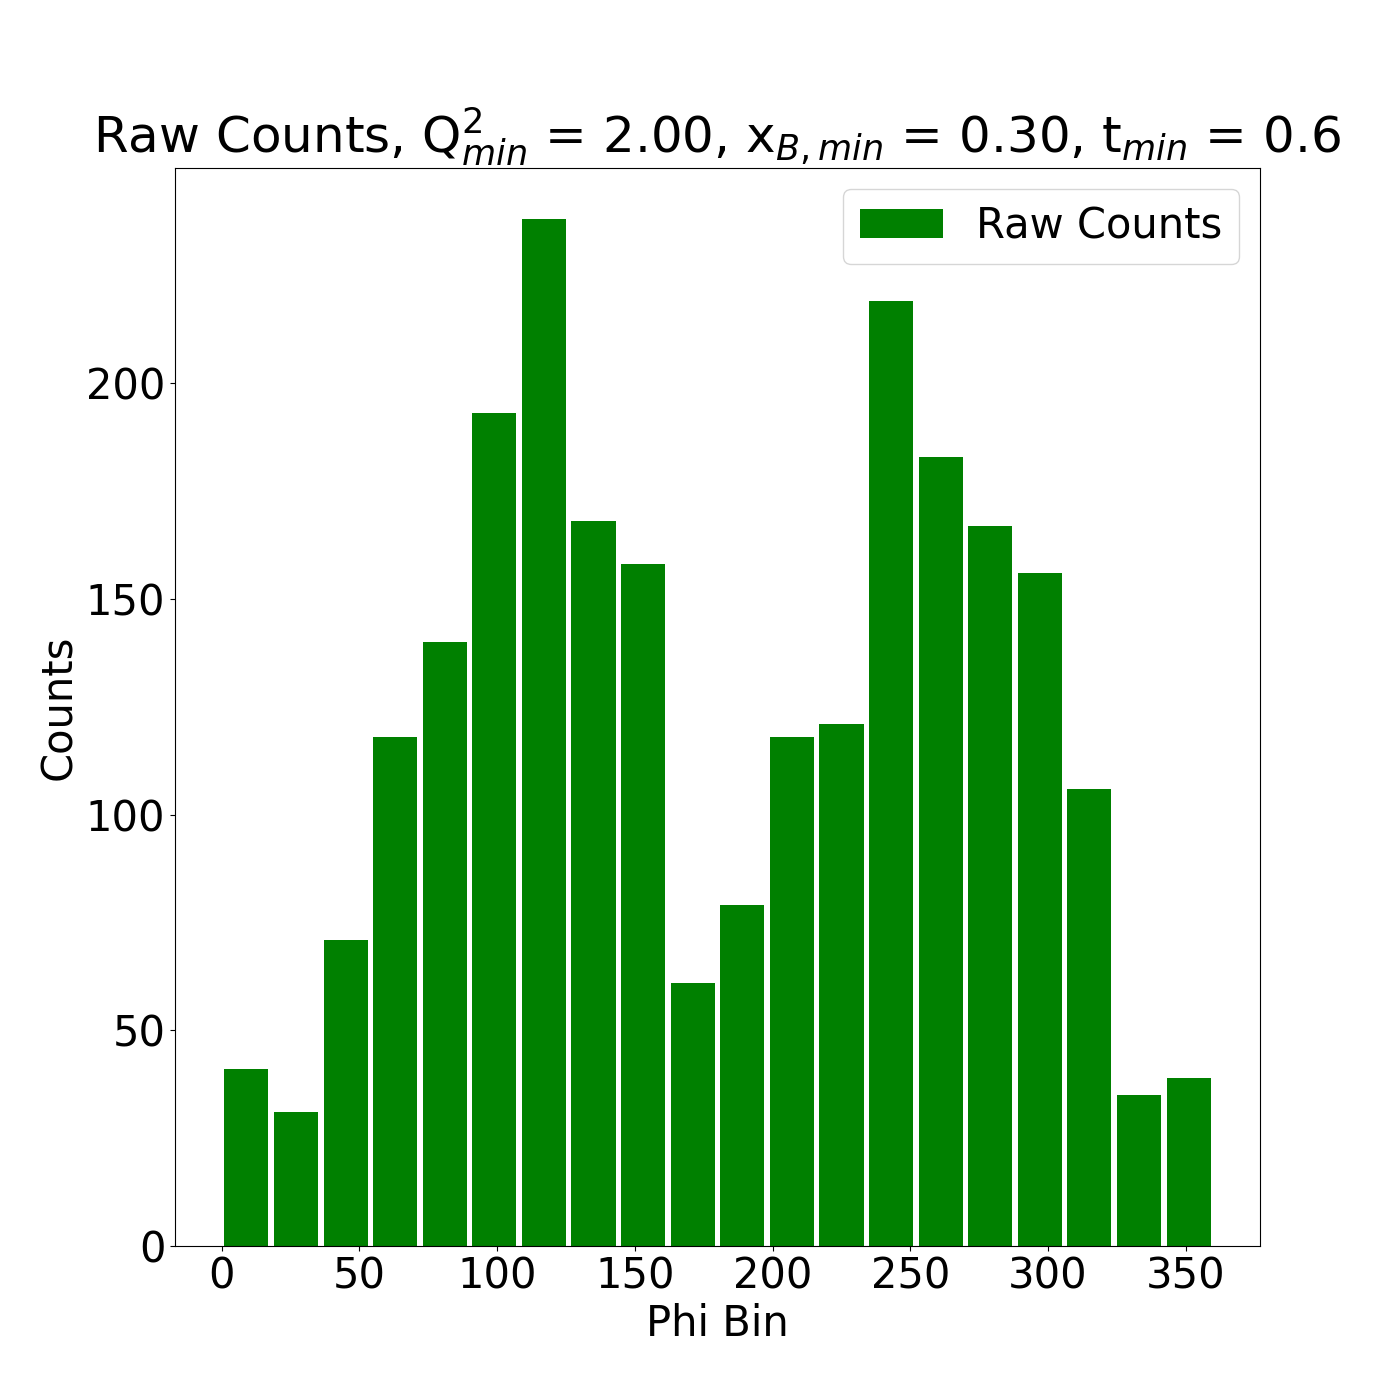
\includegraphics[width=0.5\textwidth]{Chapters/Ch4-BaseAnalysis/4_Correction_Factors/A3_a_acceptance_correction/pics/raw4.png}}
        \hfill    
        \subfloat[$N_{gen}$ and $N_{rec}$.]{\includegraphics[width=0.5\textwidth]{Chapters/Ch4-BaseAnalysis/4_Correction_Factors/A3_a_acceptance_correction/pics/acc4.png}}
        \\
        \subfloat[ 1/$\hat{\epsilon}$ = $N_{gen}$/$N_{rec}$.]{\includegraphics[width=0.5\textwidth]{Chapters/Ch4-BaseAnalysis/4_Correction_Factors/A3_a_acceptance_correction/pics/acc_3.png }}
        \hfill
        \subfloat[Acc. Corr Counts = $N_{exp}*N_{gen} / N_{rec}$ ]{\includegraphics[width=0.5\textwidth]{Chapters/Ch4-BaseAnalysis/4_Correction_Factors/A3_a_acceptance_correction/pics/final2.png}}
    
        \caption[Acceptance Correction Scheme]{Acceptance correction scheme. Experimental events (a), generated and simulated events (b) are all binned, and the ratio of reconstructed simulated events to generated events (c) is multiplied for each $N_{exp}$ to arrive at the acceptance corrected counts (d).}\label{fig:acccorr}
    %\caption[Reduced Cross Sections Across $\phi$]{Reduced Cross Sections Across $\phi$}
\end{figure}



\begin{figure}
    \centering
    \includegraphics[width=\textwidth]{Chapters/Ch4-BaseAnalysis/4_Correction_Factors/A3_a_acceptance_correction/pics/acccorr.png}
    \caption{Acceptance correction term for all bins.}
    \label{fig:acccorrdist}
\end{figure}




\subsection{Other Corrections}

    \subsubsection*{Radiative Corrections}

    Radiative corrections were estimated using simulations as described in Chapter 3. In particular, the ratio of the acceptance correction between using radiative and non-radiative generated events was taken. Sample results are shown in \figref{fig:radcorr}. 
    
    \begin{figure}[H]
    \centering

    \subfloat[]{\includegraphics[width=0.5\textwidth]{Chapters/Ch4-BaseAnalysis/4_Correction_Factors/A3_b_radiative_correction/xqt=(0.3, 1.5, 0.2).png}}
    \hfill
    \subfloat[]{\includegraphics[width=0.5\textwidth]{Chapters/Ch4-BaseAnalysis/4_Correction_Factors/A3_b_radiative_correction/xqt=(0.25, 2.0, 0.6).png}}

    \caption[Sample of Radiative Corrections ]{Radiative corrections factor for select bins.}\label{fig:radcorr}
    %\caption[Reduced Cross Sections Across $\phi$]{Reduced Cross Sections Across $\phi$}
\end{figure}

    \subsubsection*{Reconstruction Efficiency}

    Similar to radiative corrections, uncertainties in reconstruction were estimated by running simulations at different levels of current background merging (40nA, 45nA, and 55nA) and compared to the nominal 50nA datafiles. Differences were taken as a measure of systematic uncertainty. 

    \subsection*{Momentum Corrections, Smearing, and Exclusivity Cut Uncertainties}
    Uncertainties were generated for fiducial cuts / momentum corrections, smearing factors, and event selection by altering the fiducial cut areas momentum corrections and smearing factors by \pm 10\% and rerunning the analysis, and for exclusivity cuts by changing the thresholds to 2$\sigma$ (narrow) and 4$\sigma$ (wide). The differences in the resulting cross section values were taken as an estimate of uncertainty. 

    \subsection*{Finite Bin and Bin Volume Effects}
    Real data bins have finite size, so comparing counts to a differential cross section requires averaging values in a given bin. This is reasonable, assuming bins are small enough. Further, bin geometric centers do not in general align with mean bin values. This effect can be observed by taking the ratio of the generator model cross section between the bin average and bin center. Finally, the four dimension bin volume defined by the edges of each dimension might not be fully occupied by the phase space accessible in the reaction. This is addressed by taking a combination of monte carlo integration and analytical integration to correct the bin volume on the edges of acceptance. Uncertainties are propagated from the uncertainty in the generator.     
        
    \subsubsection*{Overall Normalization}

    Absolute normalization remains an ongoing effort by dedicated working groups in the CLAS collaboration. At present, we can compare the CLAS12 data to the published CLAS6 result, which contains a large number of overlapping kinematic bins. By adjusting the virtual photon flux factor and epsilon terms for the higher beam energy, we can obtain a direct comparison between the work of \parencite{Bedlinskiy2014ExclusiveCLAS} and our efforts. Published values for the reduced cross sections from the CLAS6 experiment for the DV$\pi^0$P channel are available \href{https://journals.aps.org/prc/supplemental/10.1103/PhysRevC.90.025205}{here}. Overall, there is not a large systematic shift in either direction between the CLAS12 and CLAS6 values (observe \ref{fig:combined_t0.2}-\ref{fig:combined_t1.5}). Instead, we take the difference between the two sets of data points as a measure of systematic uncertainty. This uncertainty will be removed once the current absolute normalization is validated. 


    \iffalse
    No systematic shift observed between clas6 and clas12 results, although the bins had a descrpancy that is for now included as an error untilt he absolute normazliation is better undersoot by the collaboration. The pictures only show some of it. 

    The accepted results from the CLAS6 experiment  can be used as a cross check for this work. 

    \fi

\iffalse
\subsection{Uncertainty Summary}

    Below shows a table representing sample uncertainties for a typical bin. 

    \begin{table}[ht]
    \centering
    \begin{tabular}{|l|r|}
    \hline
    \textbf{Sources} & \textbf{Typical Scale (\%)} \\
    \hline
    \textcolor{red}{SAMPLE TALBE ONLY } & NOT REAL VALUES YET \\
    Event selection — exclusivity & 11.8 \\
    Event selection — PID & 12.9 \\
    Resolution matching & 8.8 \\
    Acceptance corrections & 9.3 \\
    Background estimation & 12.8 \\
    Normalization & 10.0 \\
    Radiative Correction & 3.5 \\
    Finite bin width effect & 3.6 \\
    Reconstruction efficiency & 4.0 \\
    \hline
    \textbf{Total} & 27.0 \\
    \hline
    \end{tabular}
    \caption{Typical Scale for Different Sources}
    \label{table:example_stats}
    \end{table}

\fi
    \iffalse

    $N_rec_55/N_rec_50$ / $N_rec_50/N_rec_50$
    $N_rec_45/N_rec_50$ / $N_rec_50/N_rec_50$
    take average

    $N_rec_rad/N_rec_norad$ / $N_rec_norad/N_rec_norad$ bin by bin

    add 10\% or whatever it is norm for absolute - figure out some ratio, overall systematic shift, and then include sangbaeks note about what is wrong with it

    infold acc-corr estiamtion

    Include 30\% uncertainties for 1,2,3 uncerts

    FINIT BIN

    The advantage of finer binning is to provide improved density estimation. The
acceptance corrections and the finite bin width effects should increase with the bin
size. However, the bin size cannot be narrower than the effective resolutions in the
binning variables to minimize bin migration. Extremely small bins would not have
any statistical significance in each bin, which would lead to an invalid analysis. It is
important to determine the optimal binning.nm566+[



]
    

    The asymmetry in the phi sensititivy is expected. 
    
    
    \subsubsection*{Bin Volume Corrections}
        The bin volume is not always kinematically full, for example the a large number of bins are kinmeatically restricted, no number of ecvents could ever be found. SO, the bin shape is changed / adjusted for particularly empty bins.


    
    \subsubsection*{Overall Normalization Corrections}
        Compare to CLAS 6
        Overall normalization currently estimated by comparing to CLAS6 results, where there is overlap
    \fi


    \clearpage

\section{Bin-by-Bin Cross Sections}\label{sec:Ch4_cross_section}
    The full differential cross section for this process can be expressed by \eqref{eq:DVPiPCrossSection_theory}

        \begin{equation*}
          \recallLabel{eq:DVPiPCrossSection_theory}.
        \end{equation*}

In practice, it is easier to work with the reduced form of the cross section with the virtual photon flux factor $\Gamma$ factored out, as given by \eqref{eq:xsec_reduced}.

 \begin{equation}\label{eq:xsec_reduced}
    \frac{d^2\sigma_{\gamma^*p \rightarrow p'\pi^0}(Q^2,x_B,t,\phi_{\pi},E)}{dtd\phi} = \frac{1}{\Gamma_V(Q^2,x_B,E)} \frac{d^4\sigma_{\gamma^*p \rightarrow p'\pi^0}}{dQ^2dx_Bdtd\phi_{\pi}}.
\end{equation}

The results of this work are presented as reduced cross sections in the following pages. There were 1841 total 4-fold differential bins that passed all selection criteria. Example results are shown for sample bins in \figref{fig:redxsec_phi}. Data points are black points with error bars (black=statistical only, red = total). The black curve is a A+B$\cos(\phi)$ +C$\cos(2\phi)$ fit to the data to allow for structure extraction, the results of which are discussed in Chapter \ref{Chapter:Further Analysis}. The blue curve is the result from the CLAS6 experiment \parencite{Bedlinskiy2014ExclusiveCLAS} adjusted for the difference in beam energy. The blue band surrounding the blue curve is the approximate error for the CLAS6 result.


\iffalse
 \begin{equation}\label{xsec_red_full}
    \frac{d^2\sigma_{\gamma^*p \rightarrow p'\pi^0}}{dtd\phi} = \frac{1}{\Gamma_V(Q^2,x_B,E)} \frac{N(Q^2,x_B,t,\phi_{\pi})}{\Lumi_{int}\Delta Q^2\Delta x_B\Delta t\Delta \phi} \frac{1}{\epsilon_{ACC} \delta_{RC} \delta_{Norm} Br(\pi^0 \rightarrow \gamma \gamma)}
\end{equation}

\fi

\begin{figure}[H]
    \centering

    \subfloat[$\langle x_B \rangle$=0.23,$\langle Q^2 \rangle$=1.73 $GeV^2$,$\langle t \rangle$=0.26 $GeV^2$]{\includegraphics[width=0.5\textwidth]{Chapters/Ch4-BaseAnalysis/bin_by_bin_cross_sections/singles/xqt=(0.2, 1.5, 0.2).png}}
    \hfill
    \subfloat[$\langle x_B \rangle$=0.62,$\langle Q^2 \rangle$=7.88 $GeV^2$,$\langle t \rangle$=1.24 $GeV^2$]{\includegraphics[width=0.5\textwidth]{Chapters/Ch4-BaseAnalysis/bin_by_bin_cross_sections/singles/xqt=(0.58, 7.0, 1.0).png}}

    \caption[Reduced Cross Sections Across $\phi$]{Reduced cross sections across $\phi$ at (a) low kinematics and (b) high kinematics. Where kinematic overlap exists, the CLAS6 result \parencite{Bedlinskiy2014ExclusiveCLAS} is shown in blue with an error band (in modified form to account for beam energy differences). }\label{fig:redxsec_phi}
    %\caption[Reduced Cross Sections Across $\phi$]{Reduced Cross Sections Across $\phi$}
\end{figure}


The results are shown for bins across $x_B$, $Q^2$, and t in Figs. \ref{fig:combined_t0.2} - \ref{fig:combined_t1.5} with $x_B$ bins increasing from left to right and $Q^2$ bins increasing from bottom to top on a given page, and t bins increasing as page number increases. Note that distributions are only shown here that have enough coverage in $\phi$ to allow for a reasonable structure function curve fit. The complete cross section results are tabulated in Appendix \ref{app:Across_sections}.

\iffalse

\begin{figure}[ht]
\centering
\includegraphics[trim={14.6cm 4cm 27.2cm 4cm},clip,width=\textwidth]{Chapters/Ch4-BaseAnalysis/bin_by_bin_cross_sections/pics_screenshots/t_2.png}
\caption[Reduced Cross Section for 0.2 $GeV^2 < t <$ 0.3 $ GeV^2$]{Reduced Cross Section for 0.2 $ GeV^2 < t <$ 0.3 $GeV^2$ in bins of $x_B$ (increasing left to right) and $Q^2$ (increasing vertically upwards). }
\label{fig:combined_t0.2}
\end{figure}


\begin{figure}[ht]
\centering
\includegraphics[trim={14.1cm 4cm 27.2cm 4cm},clip,width=\textwidth]{Chapters/Ch4-BaseAnalysis/bin_by_bin_cross_sections/pics_screenshots/t_3.png}
\caption[Reduced Cross Section for 0.3 $GeV^2 < t <$ 0.4 $ GeV^2$]{Reduced Cross Section for 0.3 $ GeV^2 < t <$ 0.4 $GeV^2$.}
\label{fig:combined_t0.3}
\end{figure}


\begin{figure}[ht]
\centering
\includegraphics[trim={14.6cm 4cm 23cm 4cm},clip,width=\textwidth]{Chapters/Ch4-BaseAnalysis/bin_by_bin_cross_sections/pics_screenshots/t_4.png}
\caption[Reduced Cross Section for 0.4 $GeV^2 < t <$ 0.6 $GeV^2$]{Reduced Cross Section for 0.4 $GeV^2 < t <$ 0.6 $GeV^2$.}
\label{fig:combined_t0.4}
\end{figure}


\begin{figure}[ht]
    \centering
    \includegraphics[trim={14.8cm 4cm 18.5cm 4cm},clip,width=\textwidth]{Chapters/Ch4-BaseAnalysis/bin_by_bin_cross_sections/pics_screenshots/t_6.png}
    \caption[Reduced Cross Section for 0.6 $GeV^2 < t <$ 1.0 $GeV^2$]{Reduced Cross Section for 0.6 $GeV^2 < t <$ 1.0 $GeV^2$.}
    \label{fig:combined_t0.6}
\end{figure}


\begin{figure}[ht]
    \centering
    \includegraphics[trim={14.8cm 4cm 18.5cm 4cm},clip,width=\textwidth]{Chapters/Ch4-BaseAnalysis/bin_by_bin_cross_sections/pics_screenshots/t_10.png}
    \caption[Reduced Cross Section for 1.0 $GeV^2 < t <$ 1.5 $GeV^2$]{Reduced Cross Section for 1.0 $GeV^2 < t <$ 1.5 $GeV^2$.}
    \label{fig:combined_t1.0}
\end{figure}

\begin{figure}[ht]
    \centering
    \includegraphics[trim={18.8cm 4cm 18.5cm 4cm},clip,width=\textwidth]{Chapters/Ch4-BaseAnalysis/bin_by_bin_cross_sections/pics_screenshots/t15.png}
    \caption[Reduced Cross Section for 1.5 $GeV^2 < t <$ 2.0 $GeV^2$]{Reduced Cross Section for 1.5 $GeV^2 < t <$ 2.0 $GeV^2$.}
    \label{fig:combined_t1.5}
\end{figure}

\fi
    \clearpage
    

\iffalse

For each kinematic bin the differential cross section can be written as:

\begin{equation}
    \sigma = \frac{N_{meas}}{L \epsilon}\frac{1}{\delta}
\end{equation}

Where $\frac{N_{meas}}{L}$ is the number of events from experiment normalized by the integrated luminosity before acceptance and radiatvie corrections. $\epsilon$ = $\frac{N^{RAD}_{rec}}{{N^{RAD}_{gen}}}$ is the acceptance correction and $\delta$ is the radiative correction.



$\delta$ can be obtained by using the following:

\begin{equation}
    \delta = \frac{N^{RAD}_{gen}}{N^{NORAD}_{gen}}
\end{equation}

$\delta$ and $\epsilon$ need to be properly calculated, but for a first pass we will ignore them so we have just
\fi



